\documentclass{article}\usepackage[]{graphicx}\usepackage[]{color}
%% maxwidth is the original width if it is less than linewidth
%% otherwise use linewidth (to make sure the graphics do not exceed the margin)
\makeatletter
\def\maxwidth{ %
  \ifdim\Gin@nat@width>\linewidth
    \linewidth
  \else
    \Gin@nat@width
  \fi
}
\makeatother

\definecolor{fgcolor}{rgb}{0.345, 0.345, 0.345}
\newcommand{\hlnum}[1]{\textcolor[rgb]{0.686,0.059,0.569}{#1}}%
\newcommand{\hlstr}[1]{\textcolor[rgb]{0.192,0.494,0.8}{#1}}%
\newcommand{\hlcom}[1]{\textcolor[rgb]{0.678,0.584,0.686}{\textit{#1}}}%
\newcommand{\hlopt}[1]{\textcolor[rgb]{0,0,0}{#1}}%
\newcommand{\hlstd}[1]{\textcolor[rgb]{0.345,0.345,0.345}{#1}}%
\newcommand{\hlkwa}[1]{\textcolor[rgb]{0.161,0.373,0.58}{\textbf{#1}}}%
\newcommand{\hlkwb}[1]{\textcolor[rgb]{0.69,0.353,0.396}{#1}}%
\newcommand{\hlkwc}[1]{\textcolor[rgb]{0.333,0.667,0.333}{#1}}%
\newcommand{\hlkwd}[1]{\textcolor[rgb]{0.737,0.353,0.396}{\textbf{#1}}}%
\let\hlipl\hlkwb

\usepackage{framed}
\makeatletter
\newenvironment{kframe}{%
 \def\at@end@of@kframe{}%
 \ifinner\ifhmode%
  \def\at@end@of@kframe{\end{minipage}}%
  \begin{minipage}{\columnwidth}%
 \fi\fi%
 \def\FrameCommand##1{\hskip\@totalleftmargin \hskip-\fboxsep
 \colorbox{shadecolor}{##1}\hskip-\fboxsep
     % There is no \\@totalrightmargin, so:
     \hskip-\linewidth \hskip-\@totalleftmargin \hskip\columnwidth}%
 \MakeFramed {\advance\hsize-\width
   \@totalleftmargin\z@ \linewidth\hsize
   \@setminipage}}%
 {\par\unskip\endMakeFramed%
 \at@end@of@kframe}
\makeatother

\definecolor{shadecolor}{rgb}{.97, .97, .97}
\definecolor{messagecolor}{rgb}{0, 0, 0}
\definecolor{warningcolor}{rgb}{1, 0, 1}
\definecolor{errorcolor}{rgb}{1, 0, 0}
\newenvironment{knitrout}{}{} % an empty environment to be redefined in TeX

\usepackage{alltt}
\usepackage{amssymb,amsmath,natbib,graphicx,enumerate,subcaption,tikz,url,booktabs}

\usepackage[margin=1in]{geometry}

\newcommand{\logit}{\mbox{logit}}
\newcommand{\E}{\mathbb{E}}
\newcommand{\Prob}{\mathbb{P}}
\newcommand{\ones}{\mathbbm{1}}
\newcommand{\indic}[1]{\boldsymbol{1}_{\{ #1 \}}}
\newcommand{\mvec}{\mbox{vec}}
\newcommand{\cov}{\mbox{Cov}}
\newcommand{\eqdist}{\overset{{\cal D}}{=}}
\newcommand{\const}{\mbox{const}}
\newcommand{\iid}{\overset{iid}{\sim}}
\newcommand{\diag}{\mbox{{\bf diag}}}
\newcommand{\Diag}{\mbox{Diag}}

\newcommand{\bmu}{\boldsymbol\mu}
\newcommand{\balpha}{\boldsymbol\alpha}
\newcommand{\br}{\boldsymbol{r}}
\newcommand{\bs}{\boldsymbol{s}}
\newcommand{\by}{\boldsymbol{y}}
\newcommand{\bbeta}{\boldsymbol{\beta}}
\newcommand{\btheta}{\boldsymbol{\theta}}
\newcommand{\btau}{\boldsymbol{\tau}}
\newcommand{\bx}{\boldsymbol{x}}
\newcommand{\beps}{\boldsymbol\epsilon}

\newcommand{\cX}{{\cal X}}
\newcommand{\cA}{{\cal A}}
\newcommand{\cAmin}{{\cal A}^{\mathsmaller{-}}}

\newcommand{\vm}[1]{\mbox{vec}^\mathsmaller{-}\hspace{-0.25pc}\left(#1\right)}
\newcommand{\Imin}{I^\mathsmaller{-}}
\newcommand{\Itri}{{I^\mathsmaller{\triangle}}}

\newcommand{\deriv}[1]{\noindent {\it Derivation:} #1 $\hfill\square$}
\newcommand{\pbe}[1]{{\cal P}_{\epsilon,#1}}
\newcommand{\be}{{\cal B}_{\epsilon}}

\newcommand{\adjSet}{\{A_{k_\ell}\}_{\ell=1}^K}
\newcommand{\abSet}{\{\alpha_{k_\ell},\bbeta_{k_\ell}\}_{\ell=1}^K}
\newcommand{\bZ}{{\bf Z}}




\title{Comparing Cross Validation Methods for Penalized Cox Regression}
\author{
}
\date{ }
\IfFileExists{upquote.sty}{\usepackage{upquote}}{}
\begin{document}
\maketitle

\section*{Abstract}
Due to the semi-parametric nature of Cox Regression, conducting cross validation for Cox models has always been a challenge. While cross validation is a commonly used approach for selecting tuning parameters in penalized regression, little research has been done to study cross validation methods for penalized Cox regression. We propose two new cross-validation methods for Cox Regression, and compare them to traditional information criteria as well as a cross-validated partial likelihood approach originally proposed by Verweij et al. Our simulation studies show that, in general, cross-validation tends to be conservative (i.e., select smaller models than the ideal choice of tuning parameters) for penalized Cox regression models. However, our proposed approach of cross-validating the linear predictors generally offers the best balance of stability and performance. We also illustrate these approaches on data from studies of gene expression and progression-free survival in cancer patients.

\section{Introduction}
Cox propotional hazard regression is one of the most commonly used statistical model for analyzing data with survival outcomes. Despite its popularity, Cox model is limited by its semiparametric nature: it is challenging to evaluate the model's predictive accuracy.

In the Cox model \citep{Cox1975}, the hazard function for an observation i is given by \begin{equation}h_{i}(t) = h_{0}(t) \text{exp}( X_{i}^{T} \beta)\end{equation} where $h_{0}$ is the baseline hazard and $e^{X_{i}^{T} \beta}$ is the relative risk. Suppose there are n observations and m observed failure times, the estimation of the coefficients $\beta$s are obtained by maximizing the partial likelihood \begin{equation}L(\beta) = \prod_{j=1}^{m} \frac{\text{exp} ( X_{j}^{T} \beta)}{\sum_{ k \in R(t_{j})}\text{exp} ( X_{k}^{T} \beta)}\end{equation}, where j indexes the observed failure times and $R(t_{j})$ denotes the set of observations at risk at time $t_{j}$. As a semi-parametric model, Cox regression only gives estimations of the $\beta$ coefficients, without estimating the baseline hazard. Hence the interpretation of the Cox model is only valid in a relative sense.

Penalized Cox Regression is an extension of the regular cox regression model. Estimates of the $\beta$ coefficients are obtained by minimizing the objective function \begin{equation}  Q(\beta |X, y) = - \frac{1}{n}  \sum_{j=1}^{m} \text{log} \left \{\frac{\text{exp} ( X_{j}^{T} \beta)}{\sum_{ k \in R(t_{j})}\text{exp} ( X_{k}^{T} \beta)}) \right \} + P_{\lambda}(\beta). \end{equation} \citep{Simon2011}. The first part of the objective function is based on the partial likelihood. The second part is a penalty term that depends on some regularization parameters. In this paper, only the LASSO penalty $P_{\lambda}(\beta) = \lambda (\sum_{j} |\beta_{j}|)$ was considered. The penalized cox regression can be used for analyzing high dimensional data, where the number of covariates p $\gg$ n. A common application would be to predict the overall survival time of a particular cancer by certain gene expressions.

Selecting the tuning parameter $\lambda$ is crutial to getting LASSO estimations for $\beta$. As $\lambda$ increases, more coefficients would be set to 0 and fewer variables will be selected by the model. When $\lambda$ is too small, the model tends to be redundant. When $\lambda$ is too large, the model would be too conservative to select any variables.

One common approach for selecting the tuning parameter $\lambda$ for linear regression and logistic regression is via cross validation. The idea of K - fold cross validation is illustrated in Figure 1. The data set would be split into K folds. One fold would be treated as the test set and the other K - 1 folds as the training set. The model would first be built on the training set, then fitted to the test set to obtain cross validation error (CVE).  CVE would be calculated for each candidate $\lambda$, then the one that minimizes cross validated error would be selected.

However, for penalized cox regression, it is challenging to carry out cross validation. Since the partial likelihood of the cox model does not give estimates for the baseline, it is not meaningful to compare the coefficients if they are not estimated from different models and different observations. Only if the baseline is the same, then the coefficients can be interpreted as relative risks. This is against the idea of cross validation, which splits the data and builds models on different subsets.

\begin{figure}
    \centering
		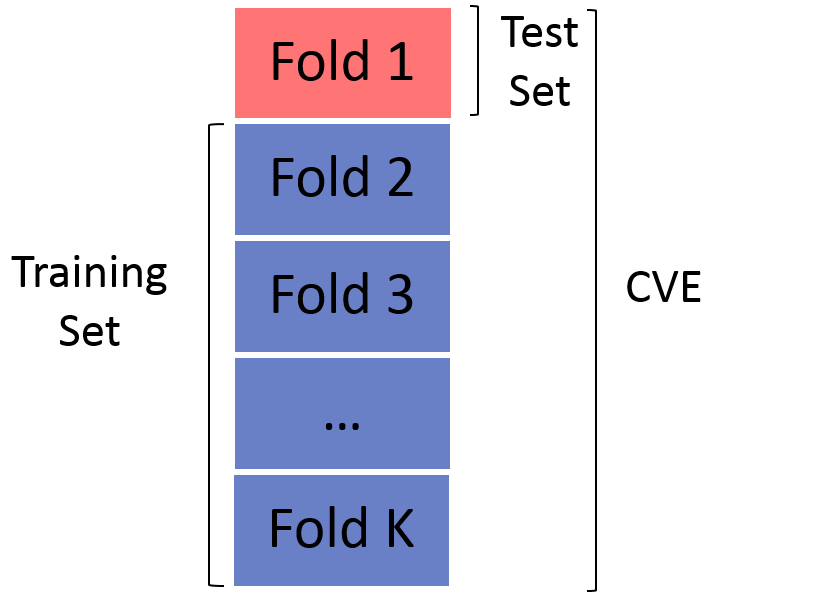
\includegraphics[height= 4cm ]{./figures/cv.png}	
    \caption{K-fold Cross Validation}
\end{figure}	

%ZZZZZZZZZZZZZ
\par The most intuitive approach to conduct cross validation in Cox regression is i) fit the model to training set then ii) calculate cross-validated partial likelihood based on the observations from the test set as a measure for the model's predictive accuracy. As will be discussed in Section 3, this approach is unstable when number of events gets small. Verweij elt. \citep{Verweij1993} proposed a stablized version of cross-validated log likehood, which has been widely used and implemented in R packages such as $\tt{glmnet}$. In this paper, we proposed two alternative ways to carry out cross validation. Instead of cross-validating over partial likelihood, we propose to cross validate over the linear predictors of the regression model and cross validate over the deviance residual \citep{Therneau1990}of the Cox model. 

\par We conducted simulation studies to compare how those methods perform in both low dimensional and high dimensional settings with LASSO penalty. We compared the two proposed methods with the cross-validated partial likelihood approaches and traditional information criteria. We showed that the linear predictor approach outperforms other cross validation approaches in various scenarios. We found out that using cross validation to select tuning parameters for LASSO penalized cox regression tends to be a conservative approach in general. Finally, we apply those methods to two high dimensional data sets with time-to-event outcomes.

\section{Methods}

  \subsection{Cross Validated Likelihood} 
Suppose a data set of n observations is split into K folds and the ith fold is left out, then a partial likelihood can be built over the K -1 folds and yields maximum likelihood estimates of the coefficients, denoted by $\hat{\beta}_{-i}$. An intuitive way to carry out cross validation is to use the partial likelihood on the test data as the cross validated error: \begin{equation}cvl = \sum_{i=1}^{K} l_{i}(\hat{\beta}_{-i})\end{equation} This is implemented in the $\tt{glmnet}$ package as the $\tt{ungrouped}$ option. 

\par An alternative way to calculate cross-validated log likelihood was proposed by Verweij elt. They defined cross-validated log likelihood of leaving the ith fold out to be \begin{equation}cvl = \sum_{i=1}^{K} \{l(\hat{\beta}_{-i}) - l_{-i}(\hat{\beta}_{-i})\}. \end{equation} When the ith fold is left out, $l(\hat{\beta}_{-i})$ is the log partial likelihood evaluated at $\hat{\beta}_{-i}$ with all k folds of observations. $l_{-i}(\hat{\beta}_{-i})$ is the log partial likelihood evaluated at $\hat{\beta}_{-i}$ with observations from the other K-1 folds. 
  
\par We refer to the first definition as ungrouped cross-validated partial likelihood (CVL) and the second definition as grouped cross-validated partial likelihood. Figure 2 illustrates the ideas of the two methods. The grouped CVL uses observations more efficiently than the ungrouped CVL. Since only the left-out fold would be used, the ungrouped cvl is unstable in practice when there are only very few observations in some folder.  


\begin{figure}
    \centering
		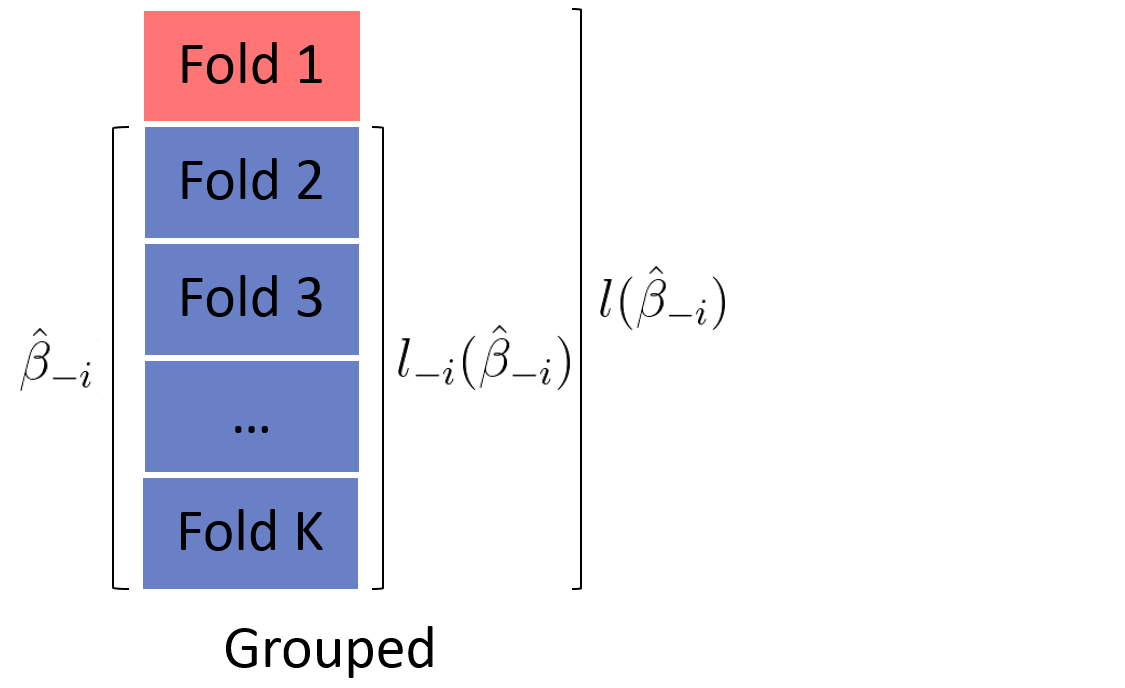
\includegraphics[height= 4cm ]{./figures/02_1.png}
		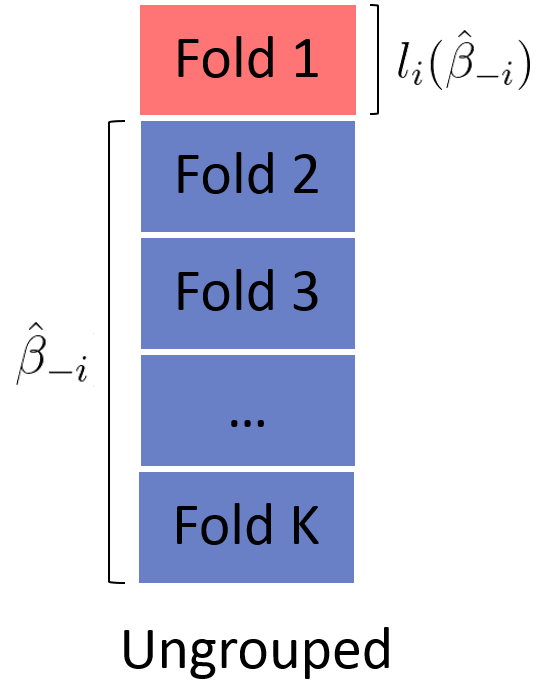
\includegraphics[height= 4cm ]{./figures/02_2.png}
    \caption{Grouped vs Ungrouped Cross Validated Likelihood}
\end{figure}	

  \subsection{Cross Validated Linear Predictors}

Besides cross validating over the partial likelihood, an alternative approach is to cross validate over the linear predictors. The data would still be split into K folds. Suppose ith fold is left out and the other K-1 folds are used as the training set to get the estimates $\hat{\beta}_{-i}$. Then the cross-validated linear predictors would be calculated based on the observations in the test set:  \begin{equation}\hat{\eta}_{-i} = X_{i}\hat{\beta}_{-i}.\end{equation} After repeating this for all K folds, a whole set of linear predictors  $\hat{\eta}_{-} = ( \hat{\eta}_{-1},  \hat{\eta}_{-2} , ...  \hat{\eta}_{-K})$ can be obtained. A partial likelihood can be built over this set of linear predictors: \begin{equation} L(\hat{\eta}_{-}) = \prod_{j=1}^{m} \frac{exp (\hat{\eta}_{-j})}{\sum_{ k \in R(t_{j})}exp (\hat{\eta}_{-k})}\end{equation}.

Cross validated error is defined as the log of $L(\hat{\eta}_{-})$. This idea of cross validating over linear predictors is implemented in the package ncvreg. For all the approaches introduced so far, they are all equivalent to each other in linear regressions. But since they are building over different baselines, they are different in cox regression.

   \begin{figure}[h]
    \centering
    \begin{minipage}[b]{0.45\textwidth}
      \centering
		  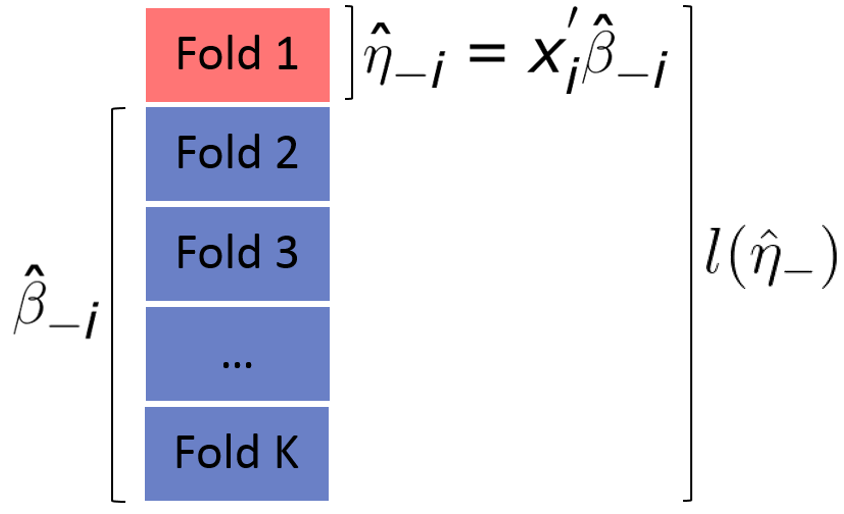
\includegraphics[height= 3.9cm ]{./figures/03.png}
      \caption{CV Linear Predictors}
     \end{minipage}
     \begin{minipage}[b]{0.45\textwidth}
      \centering
		  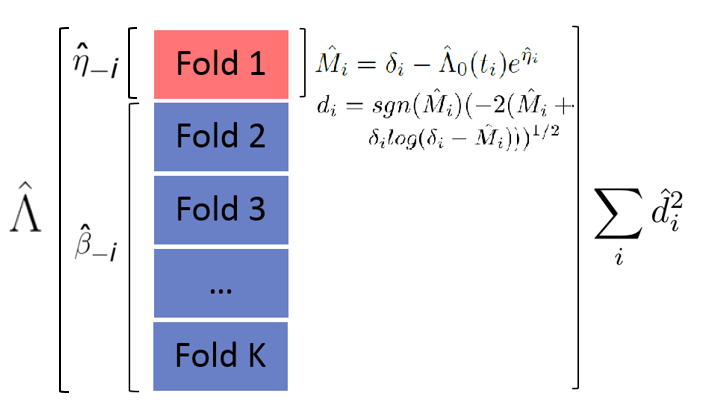
\includegraphics[height= 4.1cm ]{./figures/04_2.png}
      \caption{CV Deviance Residuals}
      \end{minipage}	
   \end{figure}	
    
  \subsection{Cross Validated Deviance Residuals}
  %Need to update this section with the new baseline estimation method%
Since the biggest challenge of conducting cross validation for cox regression is due to the missingness of baseline hazard, we propose a second approach which involves estimating the actual baseline hazard $\hat{\Lambda}_{0}$. The sum of squares of Martingale residuals is a natural candicate for evaluating the model performance using baseline hazard. Martingale residuals and its normalized form, deviance residuals, were first proposed by \citep{Therneau1990} for Cox regression model diagnostics. 

To estimate the baseline hazard, a set of linear predictors $\hat{\eta}_{-} = ( \hat{\eta}_{-1},  \hat{\eta}_{-2} , ...  \hat{\eta}_{-K})$ would be obtained in the same way as the cross validated linear predictor approach. $\hat{\eta}_{-i}$ is computed based on $\hat{\beta}_{-i}$s estimated from the training set and observations from the ith test set. With $\hat{\eta}_{-}$, a baseline hazard $\hat{\Lambda}_{0}$ can be estimated via Kalbfleisch and Prentice's method \citep{Kalbfleisch2011}. Then for each observations, the Martingale Residual can be calculated: \begin{equation}\hat{M_{i}} = \delta_{i} -\hat{\Lambda}_{0}(t_{i})e^{\hat{\eta}_{i}},\end{equation} where $\delta_{j}$ is the status of the jth observation and $t_{j}$ is the time component of the jth observation. The deviance residual can be calcualted from the Martingale Residuals: \begin{equation} d_{i} = sgn(\hat{M}_{i})(-2(\hat{M}_{i} + \delta_{i}log(\delta_{i} - \hat{M}_{i})))^{1/2}\end{equation} The sum of squares of the deviance residuals, $\sum_{i}\hat{d}_{i}^2$, would be used as the cross validated error.

As an alternative, the baseline hazard can also be estimated only based on the training set, leaving the test set as out-of-sample observations for calculating the residuals. There are two major issues with this approach. First, it would be common to run into situations where events in the test set occurred after the last event occured in the baseline, where the survival function dropped to 0. Unless those observations are treated as censored, this approach would not work. Second, there would be an extra numeric challenge for deviance residuals. Since the baseline hazard function $\hat{\Lambda}_{0}$ is a step function from 0, the cumulative hazard at the first time point from 0 is always 0. Since deviance residual contains a term $log(\delta_{i} - \hat{M}_{i})$, where $\delta_{i} - \hat{M}_{i} = \hat{\Lambda}_{0}$, this term would be negative infinity for the first time point and lead to a numeric issue for whichever fold that contains the first time point. Hence extra smoothing for the step function would be needed for this approach to work.


\section{Simulation Studies}
%reformulate this section with%
%3.1 comparison between the three methods
%3.2 discussion about stability issue for ungrouped methods
%3.3 comparison with AIC
%3.4 explaining why deviance residuals do not work well

  \subsection{Simulation Settings}
  
  Simulation studies were conducted to compare how those methods behave relative to each other. We generate data with pre-specified baseline hazard, covariate matrix X, coefficient $\beta$ and censoring mechanism. Both low dimensional and high dimentional scenarios were examined. All cross-validation methods mentioned in Section 2 were applied to the data to select the tuning parameter $\lambda$ and produce $\hat{\beta}$ estimates. Cross-validation were also compared to model selection criteria AIC and BIC.
  
  Survival times were generated from exponential distribution $h(t) = h_{0} exp(X\beta)$, conditioned on covariates. The entries in the covariate matrix $X_{n \times p}$ were independently generated from Normal (0, 1). True coefficients $\beta$  were assumed to have sparsity: $\beta_{p\times 1} = (\beta_{1},\beta_{2}, ..., \beta_{10}, 0, ..., 0)^{T}$.  Censoring status were generated based on binomial distribution.
  
  Suppose $\hat{\beta}$ is the coefficients estimated by a fitted cox model. We measure the distance between the fitted model and the true model by mean squared error $MSE = E(\hat{\beta} - \beta)^2$. For each generated data set, the $\lambda$ that has the minimal MSE is chosen as the optimal $\lambda$. Then the $\lambda$s that selected by the cross validation or information criteria would be compared to this optimal $\lambda$. If the $\lambda$ chosen by cross validation is smaller than the optimal $\lambda$, then the cross validation method would be considered liberal. If the $\lambda$ chosen by cross validation is larger than the optimal $\lambda$, then the cross validation method would be considered conservative. 
  
  \subsection{Simulation Results}
	
    \subsubsection {Stability}
   While the ungrouped cross-validated likelihood is an intuitive way to carry out cross-validation, it is quite unstable when it runs into cases where the number of observed events in some fold is really small. As is illustrated in Figure 5, cases of undefined cross-validation error would increase when censoring increases or when number of folds increases. 

\begin{figure}
    \centering
		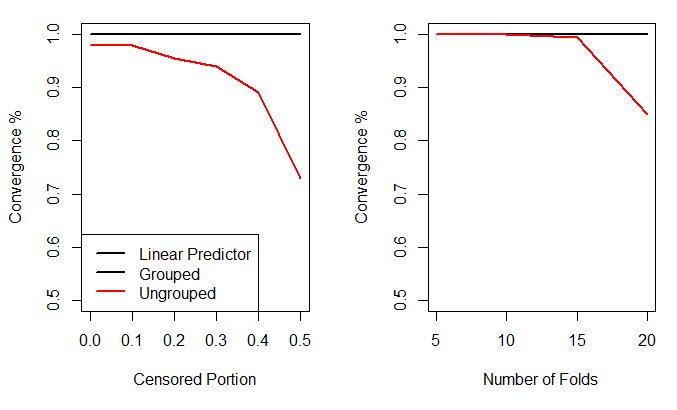
\includegraphics[height= 8cm ]{./figures/stability2.png}
    \caption{Comparing Stability}
\end{figure}	
    
    
    \subsubsection {Simulations in Low Dimensional Settings}
    
   The simulation experiments were first conducted under lower dimension settings. Number of observations n is set to be 100. Dimension of the data p is set to be 100. 200 replications were used. Censoring percentage, number of folds used in cross-validation, number of non-zero $\beta$s and the magnitude of the $\beta$000000000s were varied in several different simulation scenarios. Patterns and results shown in various simulation scenarios are consistent with one another. Figure 5 and Figure 6 illustrates one simulation scenario, where about 10$\%$ of which were set to be censored and 10 of the $\beta$s were set to be non-zero and 10 folds were used for cross validation. The x - axis of the plots are the magnitude of the non-zero $\beta$ coefficients. 
   
   \begin{figure}[h]
   \centering
    \begin{minipage}[b]{0.4\textwidth}
      \centering
		  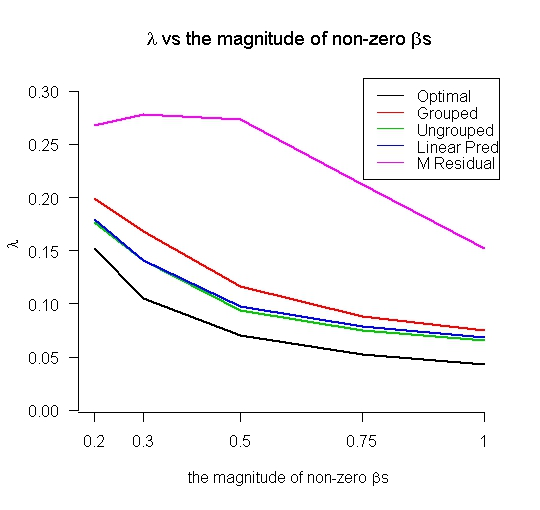
\includegraphics[height= 6cm ]{./figures/05.jpeg}
      \caption{ }
     \end{minipage}
     \begin{minipage}[b]{0.4\textwidth}
      \centering
		  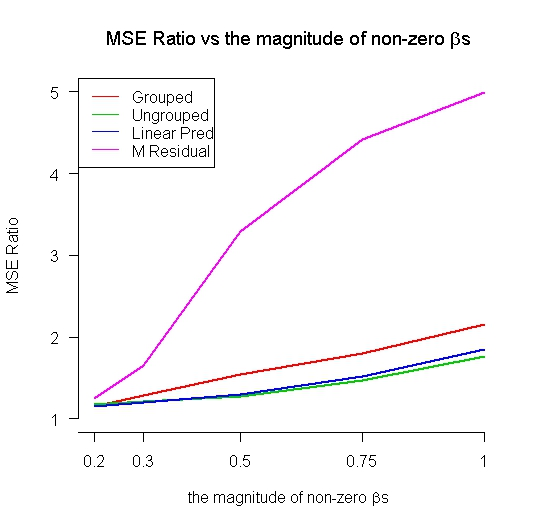
\includegraphics[height= 6cm ]{./figures/06.jpeg}
      \caption{ }
      \end{minipage}	
   \end{figure}	
   
    $\lambda$s chosen by different cross-validation methods are compared in Figure 5. All values are from taking the mean of 200 replications. The black line represents the optimal $\lambda$. All four cross validation methods consistently select $\lambda$s larger than the optimal one. Since larger $\lambda$ leads larger penalties and fewer variables are selected, all four cross validation methods seem to be conservative in terms of selecting variables. Ungrouped cross-validated log likelihood and the cross-validated linear predictor seem to be more liberal than the other two methods. The cross-validated Deviance residual is the most conservative one and its performance is quite off from the other three methods.

   Mean squared errors are compared in Figure 6. The MSEs of the cross-validation selected models are compared with the MSE of the model given by the optimal $\lambda$. The y-axis represents the ratio of the two. The ungrouped method and the linear predictor approach are outperforming the other methods and are closest to the minimal MSE.

    \subsubsection {Simulations in High Dimensional Setting}

   Simulation studies were also conducted in high dimension scenarios, where the number of observations and dimension of the covariate matrix is more similar to real genetics research. The results are shown in Table 1. Conclusions are close to what is shown in the low dimensional setting. The M- residual approach performs most conservatively. Linear predictor approach and ungrouped approach are relatively more liberal than the other approaches but still slightly more conservative than the optimal $\lambda$.
  
  \begin{table}[h]
    \centering
			\begin{tabular}{ c | c | c | c}
				CV Methods & $\lambda$ (SD) & MSE Ratio \\
				\hline \hline
				Optimal  & 0.0606 ( 0.0019 )&  / & \\ 
				Grouped  &  0.0895  ( 0.0043 )& 1.598  \\
				Ungrouped & 0.0754 ( 0.0060 )& 1.225 \\
				Linear Pred & 0.0759 ( 0.0058 )& 1.234 \\
				M Residual &0.1283 ( 0.0047 ) & 2.959
			\end{tabular}
			\caption{Simulation Results in High Dimensional Setting}
	\end{table}
  
  
  \vspace{20 mm}
    \subsubsection {Comparisons with Information Criteria}
    \par We also compared cross-validation with information criteria AIC and BIC. Simulation studies were conducted in lower dimension and higher dimension respectively. As is illustrated in Figure 7, in lower dimension, AIC tends to perform more liberal and BIC tends to perform more conservative than the optimal $\lambda$. While the cross-validation methods are also conservative, most of them are less conservative than BIC. In terms of MSE, cross-validation methods yield smaller MSE than the information criteria. In higher dimension, both BIC and AIC tend to be more liberal than the optimal $\lambda$ and yield larger MSE.

   \begin{figure}[h]
    \centering
    \begin{minipage}[b]{0.4\textwidth}
      \centering
		  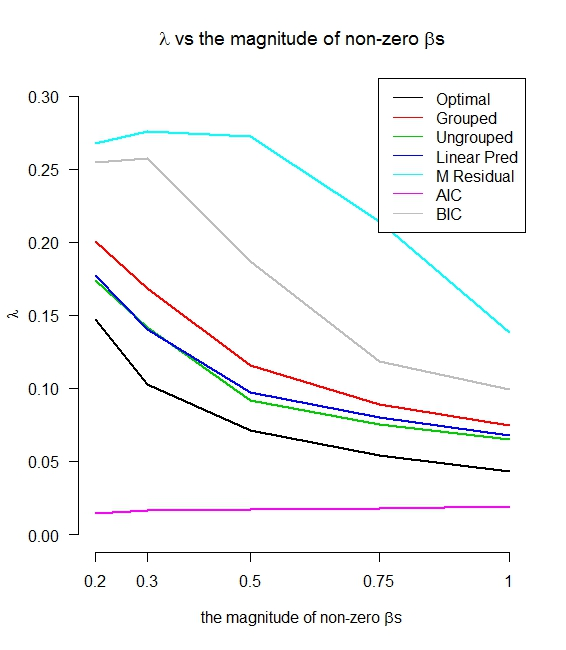
\includegraphics[height= 6cm ]{./figures/aic_01.jpeg}
      \caption{Comparison to Information Criteria in Lower Dimension}
     \end{minipage}
     \begin{minipage}[b]{0.4\textwidth}
      \centering
		  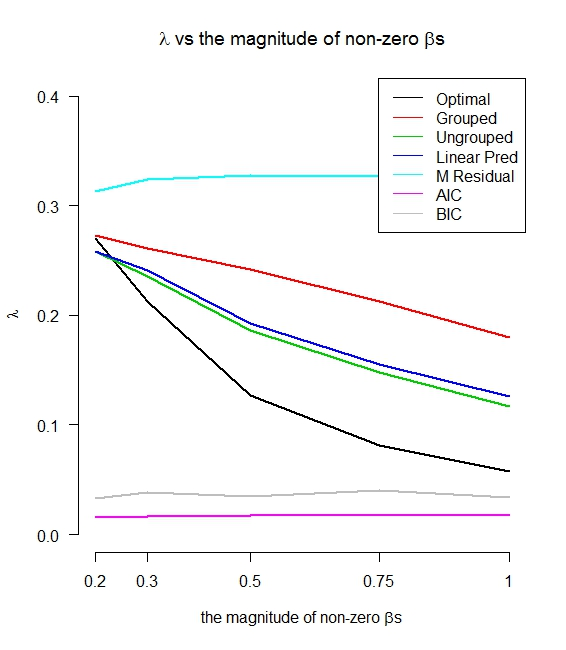
\includegraphics[height= 6cm ]{./figures/aic_02.jpeg}
      \caption{Comparison to Information Criteria in Higher Dimension}
      \end{minipage}	
   \end{figure}	
    
  
\section{Application to Real Data}

We also compared those cross validation methods when they are applied to real data sets. Unlike simulated set, we do not know the optimal $\lambda$ in the real data sets, but we can still see how those methods perform relative to each other. The first data set is a study on ovariance cancer from The Cancer Genome Atlas. The second data set is a study on lung cancer (Shedden et al 2004). The outcome of both data sets are time-to-event data.

There are 460 patients and 236 events for the ovarian cancer data set. About 40$\%$ of the observations are censored. The covariate matrix records whether or not there is mutation at the location and has dimension 12376. When we fit the penalized cox model, we first adjusted three clinical variables which is known to have large impact on survival. We first fitted these three covariates into regular cox regression and keep the linear predictors. The selection for the penalty term does not affect the estimation of those clinical variables. The results are illustrated in Table 2. The linear predictor approach has the best predictive accuracy according to AUC. 

\begin{table}[h]
\centering
  \begin{tabular}{ c | c | c | c}
				CV Methods & $\lambda$ & $log(\lambda)$ &AUC \\
				\hline \hline
				Grouped  &  0.117 & -2.14 &   0.595\\
				Ungrouped &  0.112 & -2.20 &  0.597\\
				Linear Pred &  0.085 & -2.46 &     0.607\\
				M Residual & 0.171 & -1.76 & 0.529 
	\end{tabular}
  \caption{Tuning Parameter Selected for Ovarian Cancer Data}
\end{table}


In Figure 9, the Cross Validated Error is rescaled and plotted for all four methods. A $\lambda$ will be selected when CVE curve reaches its lower point. The blue line, which represents the linear predictor approach, it has more curvature near its lowest point. It is easier to pick out the minimum point for this blue curve. Hence this approach is better at picking out signals than the other three approaches. If we look at the curve for the cross-validated Deviance Residual, there's almost no signal there.

   \begin{figure}[h]
   \centering
    \begin{minipage}[b]{0.4\textwidth}
      \centering
		  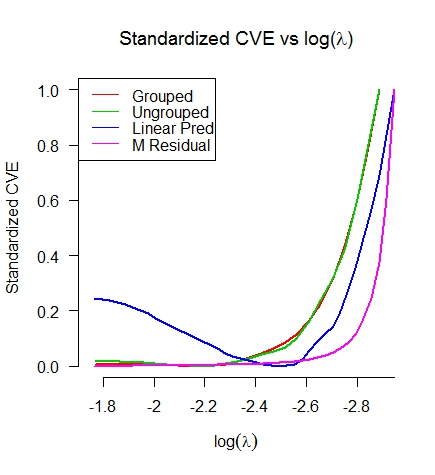
\includegraphics[height= 6cm ]{./figures/07.jpeg}
      \caption{CVE for Ovarian Cancer Data}
     \end{minipage}
     \begin{minipage}[b]{0.4\textwidth}
      \centering
		  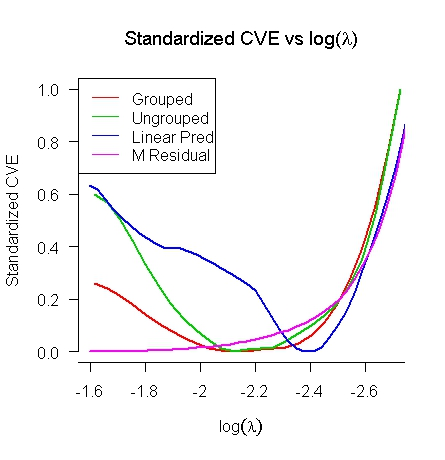
\includegraphics[height= 6cm ]{./figures/08.jpeg}
      \caption{CVE for Lung Cancer Data}
      \end{minipage}	
   \end{figure}	

In the lung cancer data set that we applied our methods to, there are 442 patients and 236 events. About 50$\%$ of the patients are censored. Again we adjusted three clinical variable before we fit the penalized regression. The results of the analysis are listed in Table 3.

			\begin{table}[h]
			\centering
			\begin{tabular}{ c | c | c | c}
				CV Methods & $\lambda$ & $log(\lambda)$ & AUC \\
				\hline \hline
				Grouped  &   0.119 & -2.12 &  0.608 \\
				Ungrouped &  0.119 & -2.12 &  0.608 \\
				Linear Pred &  0.090 & -2.41 &  0.633\\
				M Residual & 0.203 & -1.59 &  0.564
			\end{tabular}
			\caption{Tuning Parameter Selected for Lung Cancer Data}
			\end{table}
			
If we look at the CVE curve for all four of those methods, we still see that blue curve has more curvature near its lowest point. But in general, there are more signal in this lung cancer data set compared to the ovarian cancer data set.

\section{Discussion}
	\begin{itemize}
		\item 	
		\item
	\end{itemize}


\bibliographystyle{abbrvnat}
\setcitestyle{round} 
\bibliography{articles}

\end{document}
